%----------------------------------------------------------------------------------------
%	HOMEWORK ASSIGNMENT EE8744
%----------------------------------------------------------------------------------------

%----------------------------------------------------------------------------------------
%	PROLOUGE 
%----------------------------------------------------------------------------------------
\documentclass[a4paper, 11pt]{article}
\usepackage[scale=0.85]{geometry} 		% Reduce document margins
\usepackage{hyperref} 					% Required for hyperlinks i.e. e-mail %
\usepackage{titlesec} 					% Used to customize the \section command
\usepackage[T1]{fontenc}				% Used to have both Bold and Small caps in heading
\usepackage{amsmath}					% Used to write equations
\usepackage{amssymb}					% Used to write math symbols e.g. R = real number set
\usepackage{autobreak}
\usepackage{graphicx}					% Used to include images
\usepackage{tabularx} 					% For custom table %
\usepackage{mathtools}					% For define notation
\usepackage{bbm}
\allowdisplaybreaks
%----------------------------------------------------------------------------------------
%	CUSTOM MACRO DEFINITION AND ENVIRONMENT MODIFICATION
%----------------------------------------------------------------------------------------
\titleformat{\section}{\bfseries\Large\scshape\filcenter}{}{0em}{}[{\titlerule[1pt]}] % Text formatting of sections
\titlespacing{\section}{0pt}{3pt}{3pt} % Spacing around sections
\pagestyle{empty} % Removes page numbering
\newcommand{\xVec}{\ensuremath{\boldsymbol{x}}}
\newcommand{\wVec}{\ensuremath{\boldsymbol{w}}}
\newcommand{\muVec}{\ensuremath{\boldsymbol{\mu}}}
\newcommand{\mVec}{\ensuremath{\boldsymbol{m}}}
\newcommand{\sVec}{\ensuremath{\boldsymbol{S}}}
\newcommand{\sigmaVec}{\ensuremath{\boldsymbol{\sigma}}}
\newcommand{\SigmaVec}{\ensuremath{\boldsymbol{\Sigma}}}
\DeclareMathOperator*{\minimize}{minimize}
%----------------------------------------------------------------------------------------
%	MAIN BODY
%----------------------------------------------------------------------------------------
\begin{document}
	%----------------------------------------------------------------------------------------
%	HEADER
%----------------------------------------------------------------------------------------
\section{HW 3}
\begin{tabularx}{\textwidth}{l}
	\hspace*{-0.8cm}\large\textsc{Arnab Dey}\\
	\hspace*{-0.8cm}Student ID: 5563169\\
	\hspace*{-0.8cm}Email: dey00011@umn.edu\\
\end{tabularx}
\bigskip
\par
    %----------------------------------------------------------------------------------------
%	SOLUTION 1
%----------------------------------------------------------------------------------------
\subsection*{Problem 1}
In case of a balanced three-phase capacitive circuit with effective series resistance $R$, we can get the following dynamics from KVL in time domain:
\begin{align}\label{eq:q1_dyn_eqn}
	C\frac{\text{d}}{\text{d}t}
	\begin{bmatrix}
		v_a\\v_b\\v_c
	\end{bmatrix}-RC\frac{\text{d}}{\text{d}t}\begin{bmatrix}
		i_a\\i_b\\i_c
	\end{bmatrix} &= \begin{bmatrix}
		i_a\\i_b\\i_c
	\end{bmatrix}.
\end{align}
We know that, for a vector $[x_a\ x_b\ x_c]^T$ represented in $3$-phase domain can be transformed to d-q axis (at an angle $\theta_d$) with amplitude preservation in the following way:
\begin{align*}
\begin{bmatrix}
x_d\\x_q
\end{bmatrix} &= \frac{2}{3}\Gamma_{dq}\begin{bmatrix}
x_a\\x_b\\x_c
\end{bmatrix},
\end{align*}
where,
\begin{align*}
\Gamma_{dq} &= \begin{bmatrix}
\cos \theta_d & \cos (\theta_d - \frac{2\pi}{3}) & \cos (\theta_d + \frac{2\pi}{3})\\
-\sin \theta_d & -\sin (\theta_d - \frac{2\pi}{3}) & -\sin (\theta_d + \frac{2\pi}{3})
\end{bmatrix}.
\end{align*}
The inverse transform can be shown to be:
\begin{align*}
\begin{bmatrix}
x_a\\x_b\\x_c
\end{bmatrix} &= \Gamma_{dq}^T \begin{bmatrix}
x_d\\x_q
\end{bmatrix}.
\end{align*}
Let us derive $\frac{\text{d}}{\text{d}t}\Gamma_{dq}^T$ first as it will be required later.
\begin{align*}
\frac{\text{d}}{\text{d}t} \Gamma_{dq}^T &= \dot{\theta_d}\begin{bmatrix}
-\sin \theta_d & \cos \theta_d\\
-\sin (\theta_d-\frac{2\pi}{3}) & -\cos (\theta_d-\frac{2\pi}{3})\\
-\sin (\theta_d+\frac{2\pi}{3}) & -\cos (\theta_d+\frac{2\pi}{3}) 
\end{bmatrix} \\
&= \dot{\theta_d} \Gamma_{dq}^T \begin{bmatrix}
0 & -1\\1 & 0
\end{bmatrix}.
\end{align*}
Therefore, from Eq.~\ref{eq:q1_dyn_eqn},
\begin{align*}
	&C\frac{\text{d}}{\text{d}t}\left(\Gamma_{dq}^T\begin{bmatrix}
		v_d\\v_q
	\end{bmatrix}\right)-RC\frac{\text{d}}{\text{d}t}\left(\Gamma_{dq}^T\begin{bmatrix}
		i_d\\i_q
	\end{bmatrix}\right) = \Gamma_{dq}^T\begin{bmatrix}
		i_d\\i_q
	\end{bmatrix}\\
	\implies & C\dot{\theta_d}\Gamma_{dq}^T\begin{bmatrix}
		0&-1\\1&0
	\end{bmatrix}\begin{bmatrix}
		v_d\\v_q
	\end{bmatrix}+C\Gamma_{dq}^T\begin{bmatrix}
		\dot{v_d}\\\dot{v_q}
	\end{bmatrix} - RC \dot{\theta_d}\Gamma_{dq}^T\begin{bmatrix}
		0&-1\\1&0
	\end{bmatrix}\begin{bmatrix}
		i_d\\i_q
	\end{bmatrix}-RC\Gamma_{dq}^T\begin{bmatrix}
		\dot{i_d}\\\dot{i_q}
	\end{bmatrix} = \Gamma_{dq}^T\begin{bmatrix}
		i_d\\i_q
	\end{bmatrix}\\
	\implies & C\dot{\theta_d}\begin{bmatrix}
		-v_q\\v_d
	\end{bmatrix}+C\begin{bmatrix}
		\dot{v_d}\\\dot{v_q}
	\end{bmatrix}-RC\dot{\theta_d}\begin{bmatrix}
		-i_q\\i_d
	\end{bmatrix}-RC\begin{bmatrix}
		\dot{i_d}\\\dot{i_q}
	\end{bmatrix} = \begin{bmatrix}
		i_d\\i_q
	\end{bmatrix}\\
	\implies & C\left(\begin{bmatrix}
		\dot{v_d}\\\dot{v_q}
	\end{bmatrix}-R\begin{bmatrix}
		\dot{i_d}\\\dot{i_q}
	\end{bmatrix}\right)+C\dot{\theta_d}\begin{bmatrix}
		-v_q\\v_d
	\end{bmatrix}-RC\dot{\theta_d}\begin{bmatrix}
		-i_q\\i_d
	\end{bmatrix} = \begin{bmatrix}
		i_d\\i_q
	\end{bmatrix}.
\end{align*}
Therefore, the dynamics in dq domain can be written as:
\begin{align*}
	C\frac{\text{d}}{\text{d}t}\left(v_d-i_dR\right)-C\dot{\theta_d}v_q+RC\dot{\theta_d}i_q &= i_d,\\
	C\frac{\text{d}}{\text{d}t}\left(v_q-i_qR\right)+C\dot{\theta_d}v_d-RC\dot{\theta_d}i_d &= i_q.
\end{align*}

    %%----------------------------------------------------------------------------------------
%	SOLUTION 2.1
%----------------------------------------------------------------------------------------
\subsection*{Problem 2.1}

    %%----------------------------------------------------------------------------------------
%	SOLUTION 3.1
%----------------------------------------------------------------------------------------
\subsection*{Problem 3.1}

    %%----------------------------------------------------------------------------------------
%	SOLUTION 4.i
%----------------------------------------------------------------------------------------
\subsection*{Problem 4.i}
The time domain dynamics of the circuit is given by:
\begin{align*}
	\begin{bmatrix}
		v_t^a\\v_t^b\\v_t^c
	\end{bmatrix} &= L \frac{\text{d}}{\text{d}t}\begin{bmatrix}
		i_a\\i_b\\i_c
	\end{bmatrix} + R \begin{bmatrix}
		i_a\\i_b\\i_c
	\end{bmatrix}+\begin{bmatrix}
		v_0^a\\v_0^b\\v_0^c
	\end{bmatrix}.
\end{align*}
Converting them to d-q domain (at an angle $\theta_d=\omega_d t$) as illustrated in Q3, we get:
\begin{align*}
	&\Gamma_{dq}^T \begin{bmatrix}
		v_t^d\\v_t^q
	\end{bmatrix} = L\frac{\text{d}}{\text{d}t}\left(\Gamma_{dq}^T\begin{bmatrix}
		i_d\\i_q
	\end{bmatrix}\right)+R\Gamma_{dq}^T\begin{bmatrix}
		i_d\\i_q
	\end{bmatrix}+\Gamma_{dq}^T\begin{bmatrix}
		v_0^d\\v_0^q
	\end{bmatrix}\\
	\implies & \Gamma_{dq}^T\begin{bmatrix}
		v_t^d\\v_t^q
	\end{bmatrix} = L\dot{\theta_d}\Gamma_{dq}^T\begin{bmatrix}
		0 & -1\\1 & 0
	\end{bmatrix}\begin{bmatrix}
		i_d\\i_q
	\end{bmatrix}+L\Gamma_{dq}^T\begin{bmatrix}
		\dot{i_d}\\\dot{i_q}
	\end{bmatrix}+R\Gamma_{dq}^T\begin{bmatrix}
		i_d\\i_q
	\end{bmatrix}+\Gamma_{dq}^T\begin{bmatrix}
		v_0^d\\v_0^q
	\end{bmatrix}\\
	\implies & \begin{bmatrix}
		v_t^d\\v_t^q
	\end{bmatrix} = L\omega_d\begin{bmatrix}
		-i_q\\i_d
	\end{bmatrix}+L\begin{bmatrix}
		\dot{i_d}\\\dot{i_q}
	\end{bmatrix}+R\begin{bmatrix}
		i_d\\i_q
	\end{bmatrix}+\begin{bmatrix}
		v_0^d\\v_0^q
	\end{bmatrix}.
\end{align*}
Converting the above equations in block diagrams along with feedback control and following Fig.~3 in the question for point of feed forward, we get the following block diagram shown in Fig.~\ref{fig:q4_block_dia} in dq domain as requested in the question.
%%%%%%%%%%%%%%%%%%%%%%% BLOCK DIAGRAM %%%%%%%%%%%%%%%%%%%%%
\begin{figure}[!h]
	\centering
	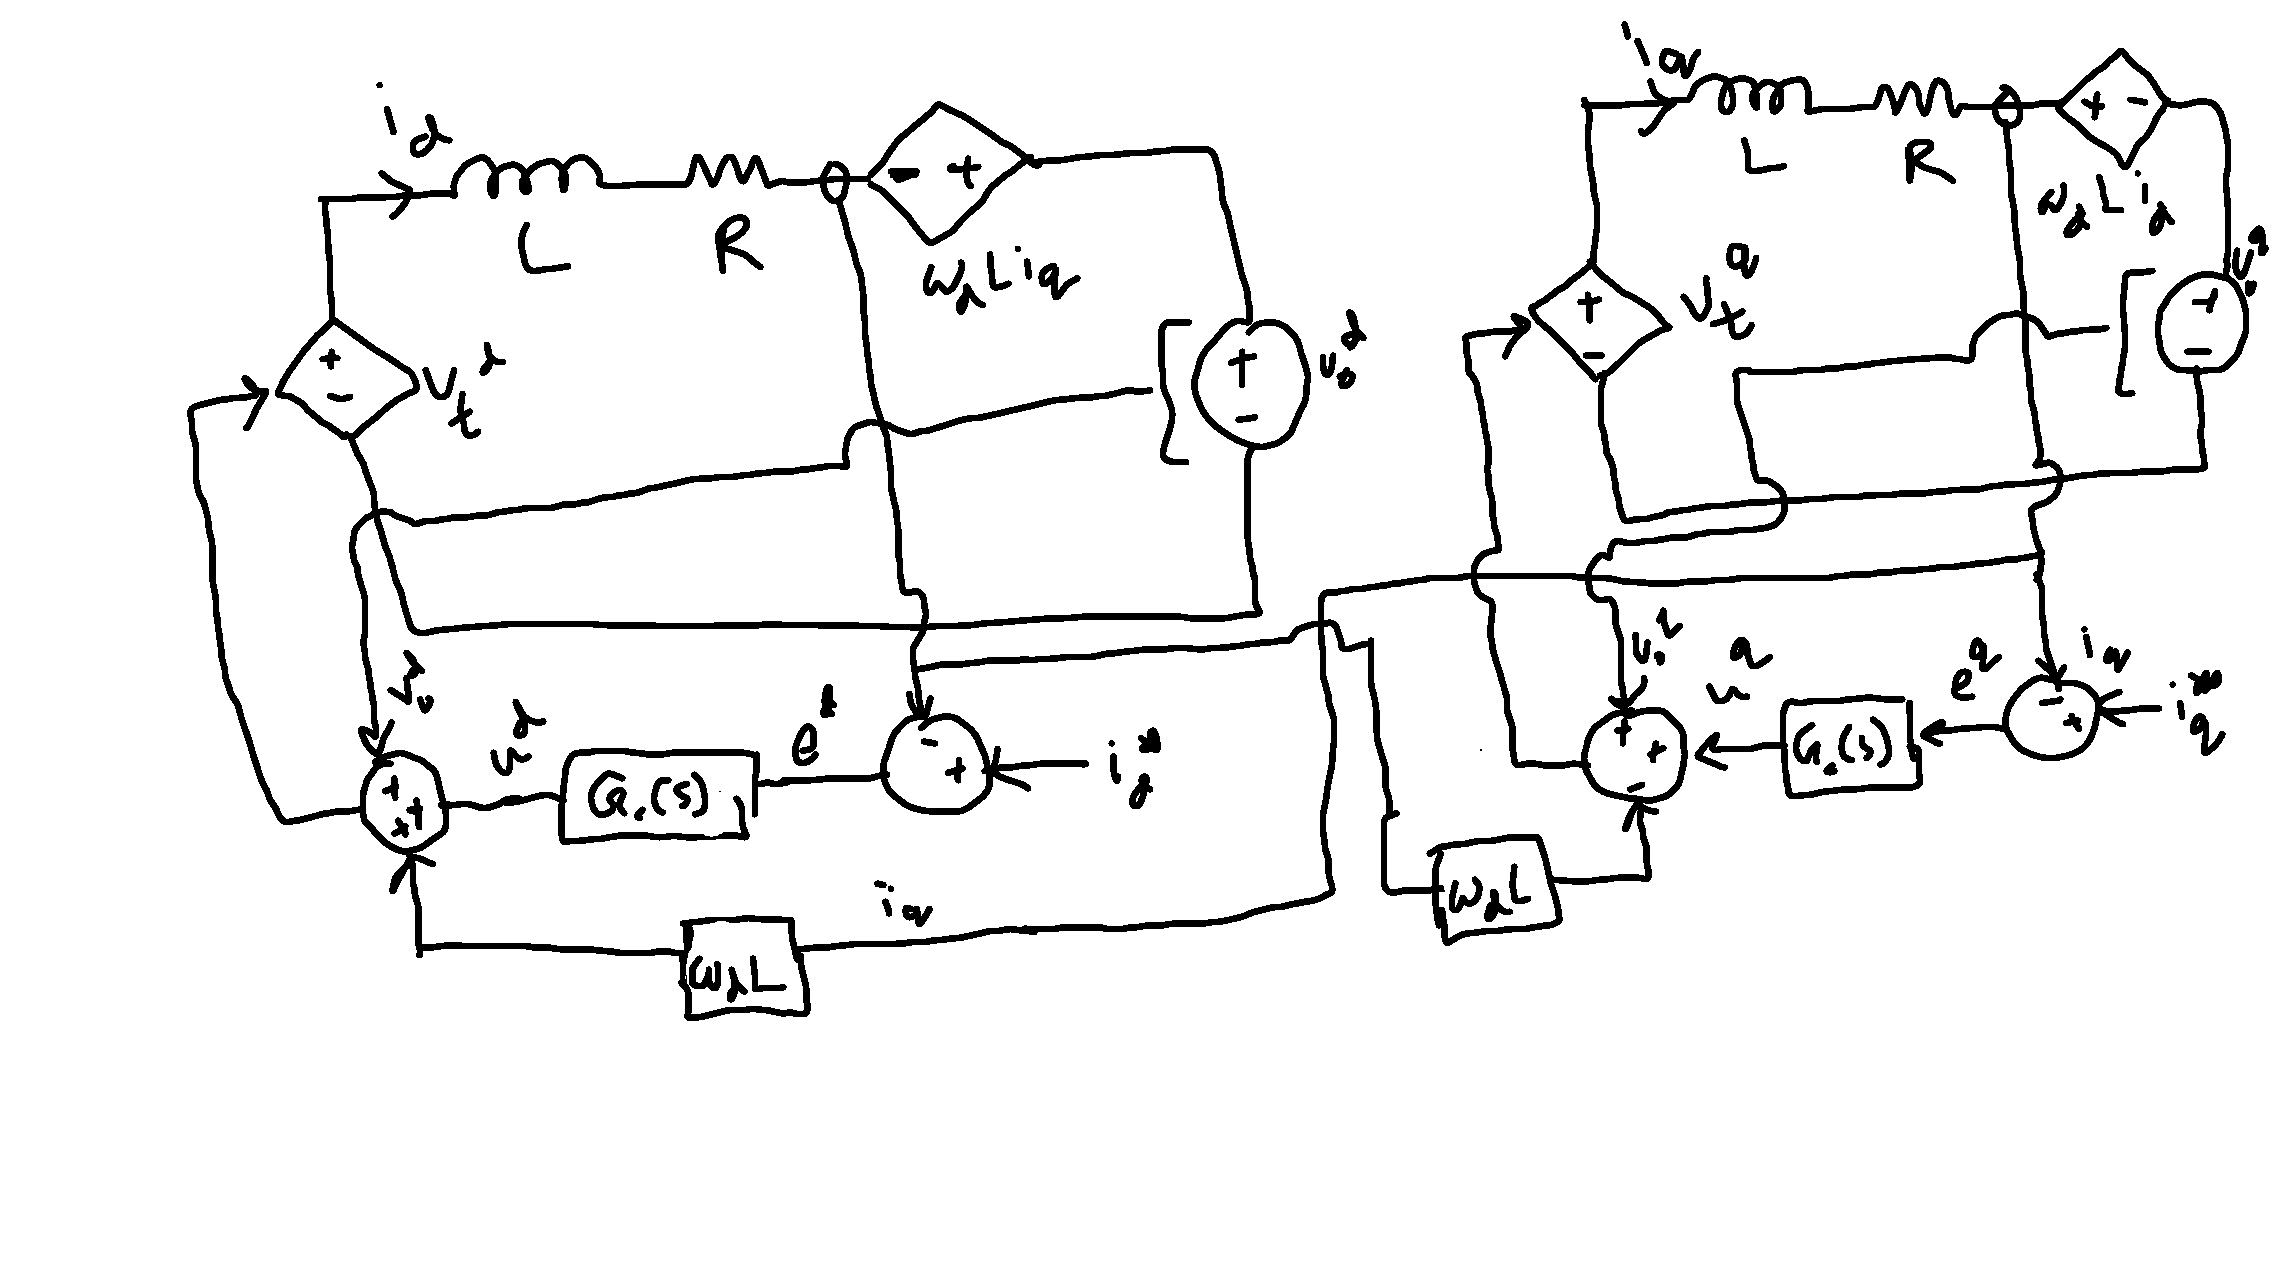
\includegraphics[scale=0.4,trim={2cm 4cm 0cm 0cm},clip]{q4_block_dia.pdf}
	\caption{Q4: Inverter feedback control block diagram}
	\label{fig:q4_block_dia}
\end{figure}
%----------------------------------------------------------------------------------------
%	SOLUTION 4.ii
%----------------------------------------------------------------------------------------
\subsection*{Problem 4.ii}
To derive the closed-loop transfer functions $\frac{i_{dq}(s)}{i_{dq}^*(s)}$, we need to ignore the cross-coupling terms and $v_{dc}$ in Fig.~3 (in the question). Then we can get the following the block diagram for $i_d(s)$ (similar diagram for $i_q(s)$ too) as shown in Fig.~\ref{fig:q4_tf}:
%%%%%%%%%%%%%%%%%%%%%%% TRANSFER FUNCTION %%%%%%%%%%%%%%%%%%%%%
\begin{figure}[!h]
	\centering
	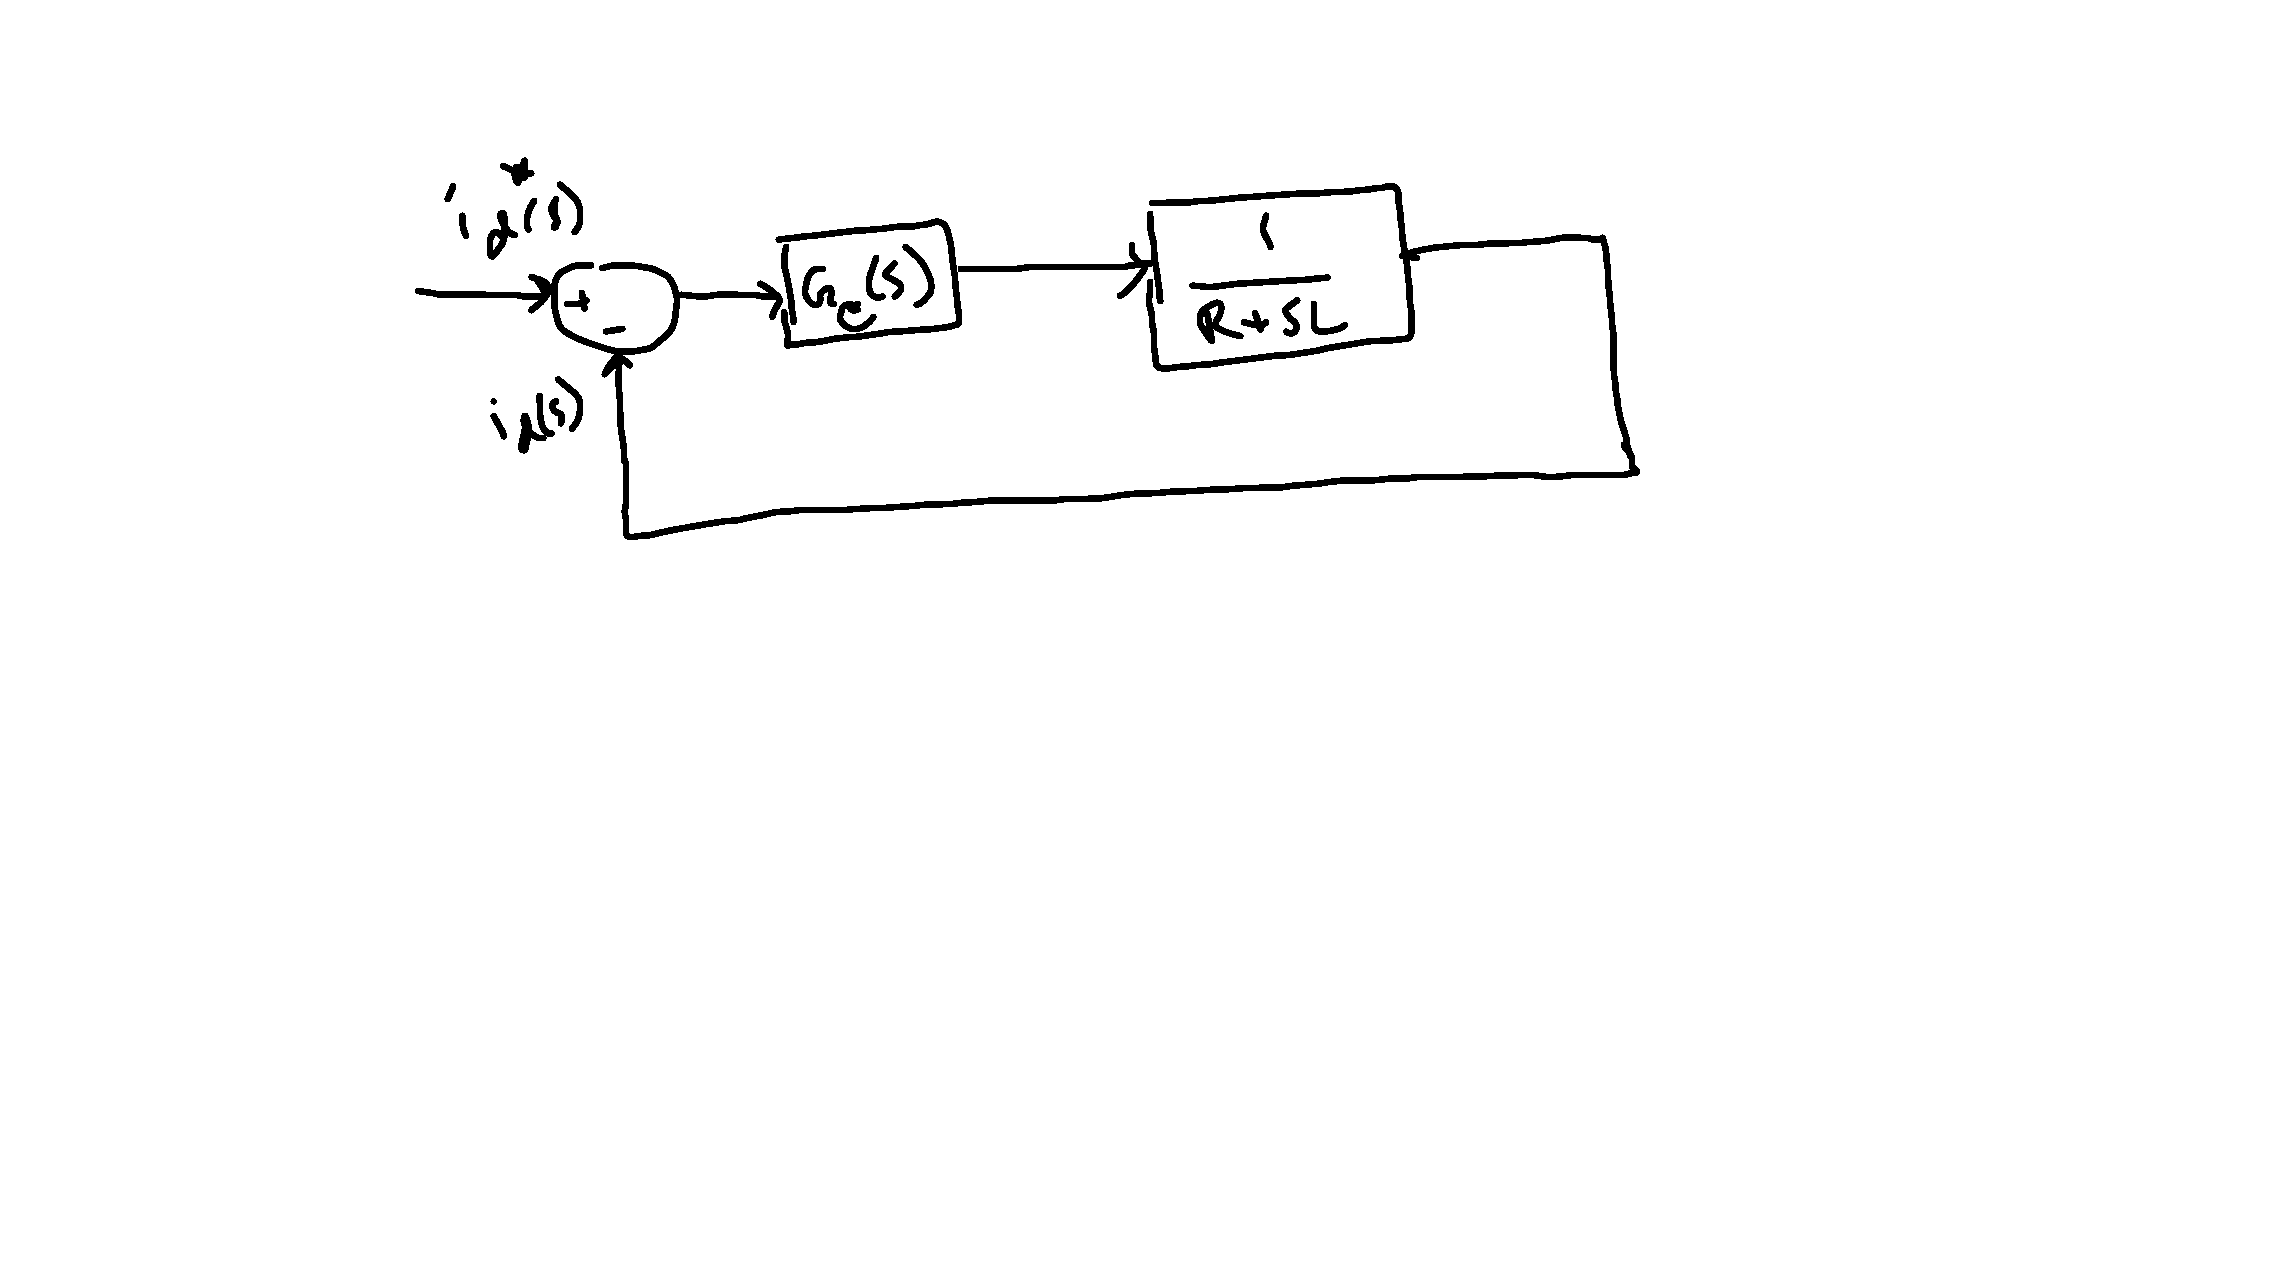
\includegraphics[scale=0.4,trim={2cm 12cm 0cm 0cm},clip]{q4_tf.pdf}
	\caption{Q4: Block diagram to derive current transfer function}
	\label{fig:q4_tf}
\end{figure}

Considering $G_c(s)=(k_p+k_i/s)$, we can derive the transfer function as follows:
\begin{align}\label{eq:q4_tf}
	H(s) &= \frac{i_d(s)}{i_d^*(s)} \nonumber\\
	&= \frac{G_c(s)/(R+sL)}{1+G_c/(R+sL)} \nonumber\\
	&= \frac{G_c(s)}{(R+sL)+G_c(s)} \nonumber\\
	&= \frac{k_p+k_i/s}{(k_p+k_i/s)+(R+sL)}.
\end{align}
%----------------------------------------------------------------------------------------
%	SOLUTION 4.iii
%----------------------------------------------------------------------------------------
\subsection*{Problem 4.iii}
From Eq.~\ref{eq:q4_tf}, we get,
\begin{align}\label{eq:q4_iii_a}
	H(s) &= \frac{sk_p+k_i}{s^2L+s(R+k_p)+k_i} \nonumber\\
	&= \frac{1}{\frac{s^2L}{sk_p+k_i}+\frac{s(R+k_p)}{sk_p+k_i}+\frac{k_i}{sk_p+k_i}}
\end{align}
Equating denominator of Eq.~\ref{eq:q4_iii_a} with that of desired transfer function $\frac{1}{1+\tau s}$, we get:
\begin{align*}
	&\frac{s^2L}{sk_p+k_i}+\frac{s(R+k_p)}{sk_p+k_i}+\frac{k_i}{sk_p+k_i} = (1+\tau s)\\
	\implies & s^2L+s(R+k_p)+k_i = s^2 \tau k_p + s(k_p+\tau k_i)+k_i.
\end{align*}
Equating corresponding coefficients of $s$, we get:
\begin{align*}
	L &= \tau k_p \implies \tau = \frac{L}{k_p}\\
	R+k_p &= k_p+\tau k_i \implies \tau = \frac{R}{k_i}.
\end{align*}
Therefore,
\begin{align*}
	&\frac{L}{k_p} = \frac{R}{k_i}\\
	\implies & \frac{L}{R} = \frac{k_p}{k_i}.
\end{align*}
Similarly, we can prove the \textit{only if} part as follows.\\
Let, $\frac{L}{R}=\frac{k_p}{k_i}=c$. Also denote $\tau \coloneqq \frac{R}{k_i}$. Then $\tau = \frac{L}{k_p}$ also. From Eq.~\ref{eq:q4_tf},
\begin{align*}
	H(s) &= \frac{k_p+k_i/s}{(k_p+k_i/s)+(R+sL)}\\
	&= \frac{1}{1+\frac{R+sL}{k_p+k_i/s}}\\
	&= \frac{1}{1+\frac{(R/k_i)+s(L/k_i)}{(k_p/k_i)+(1/s)}}\\
	&= \frac{1}{1+\frac{\tau+s\frac{L}{k_p}\frac{k_p}{k_i}}{c+(1/s)}}\\
	&= \frac{1}{1+\frac{\tau + sc\frac{L}{k_p}}{c+(1/s)}}\\
	&= \frac{1}{1+\frac{s\tau+s^2c\tau}{sc+1}}\\
	&= \frac{1}{1+\tau s}.
\end{align*}

    %%----------------------------------------------------------------------------------------
%	SOLUTION 5
%----------------------------------------------------------------------------------------
\subsection*{Problem 5}
It is given that the wind power random variable $V$ follows uniform distribution as follows
\begin{align*}
	V \sim U(5,20).
\end{align*}
Therefore the PDF and CDF is given by
\begin{align*}
	f_V(v) &= \begin{cases}
		\frac{1}{15},\ v \in [5,20]\\
		0,\ \text{otherwise}
	\end{cases}\\
	F_V(v) &= \begin{cases}
		0,\ v < 5,\\
		\frac{v-5}{15},\ v \in [5,20],\\
		1,\ v > 20.
	\end{cases}
\end{align*}
Now, it is given that
\begin{align*}
	V_c &= 0\\
	V_r &= 5\\
	V_F &= 15\\
	P_{rated} &= 1000 \text{ W}.
\end{align*}
Therefore,
\begin{align*}
	P(v\geq 5) &= 1-F_V(5) = 1\\
	P(v \geq 15) &= 1-F_V(15) = 0.33.
\end{align*}
It is not clear if the question asks for annual energy yield at rated power. I assume that the question asks for annual energy yield at rated power. Therefore, annual energy that the wind turbine would generate is
\begin{align*}
	8670(1-0.33)(1000) = 5.87\times 10^6 \text{ W-h}.
\end{align*}
    %%----------------------------------------------------------------------------------------
%	SOLUTION 6.1
%----------------------------------------------------------------------------------------
\subsection*{Problem 6.1}
The current voltage equation can be written as:
\begin{align}\label{eq:q6_cur_vol}
	\begin{bmatrix}
		I\\I_{N+1}
	\end{bmatrix} &= \begin{bmatrix}
		Y & \overline{Y}\\
		\overline{Y}^T & y
	\end{bmatrix}\begin{bmatrix}
		V\\V_0e^{j\theta_0}
	\end{bmatrix}
\end{align}
Therefore,
\begin{align*}
	\begin{bmatrix}
		Y & \overline{Y}\\
		\overline{Y}^T & y
	\end{bmatrix}^{-1}\begin{bmatrix}
		I\\I_{N+1}
	\end{bmatrix} &= \begin{bmatrix}
		V\\V_0e^{j\theta_0}
	\end{bmatrix}.
\end{align*}
It can be proved that the inverse exists as $Y$ is the Y-bus matrix of the system (Not proving to keep the answer concise). Also, $Y^{-1}$ and $y^{-1}$ exist. Now, using partition matrix inversion lemma,
\begin{align*}
	\begin{bmatrix}
		(Y-\overline{Y}y^{-1}\overline{Y}^T)^{-1} & -Y^{-1}\overline{Y}(y-\overline{Y}^TY^{-1}\overline{Y})^{-1}\\
		-y^{-1}\overline{Y}^T(Y-\overline{Y}y^{-1}\overline{Y}^T)^{-1} & (y-\overline{Y}^TY^{-1}\overline{Y})^{-1}
	\end{bmatrix}\begin{bmatrix}
		I\\I_{N+1}
	\end{bmatrix} &= \begin{bmatrix}
		V\\V_0e^{j\theta_0}
	\end{bmatrix}.
\end{align*}
Now, it is given that $I = 0_{N}$ and $V_0e^{j\theta_0} = 1$. Under this condition, $V$ is denoted by $V^{nom}$. Therefore from the above equation, equating left hand side and right hand side, we get,
\begin{align*}
	-Y^{-1}\overline{Y}(y-\overline{Y}^TY^{-1}\overline{Y})^{-1}I_{N+1} &= V^{nom}\\
	(y-\overline{Y}^TY^{-1}\overline{Y})^{-1}I_{N+1} &= 1\\
	\implies I_{N+1} &= (y-\overline{Y}^TY^{-1}\overline{Y}).
\end{align*}
Therefore, solving for $V^{nom}$, we get
\begin{align*}
	V^{nom} &= -Y^{-1}\overline{Y}(y-\overline{Y}^TY^{-1}\overline{Y})^{-1}(y-\overline{Y}^TY^{-1}\overline{Y})\\
	&= -Y^{-1}\overline{Y}.
\end{align*}
NOw, it is given that there are no shunt elements in the system. Therefore, each row sum of $Y$ and $\overline{Y}$ must be zero (from the structure of Y-bus matrix). Therefore, $Y\mathbbm{1}_N + \overline{Y}=0$, \textit{i.e.} $\overline{Y} = -Y\mathbbm{1}_N$. Plugging in the expression of $\overline{Y}$ in the above equation, we get
\begin{align*}
	V^{nom} &= Y^{-1}Y\mathbbm{1}_N\\
	&= \mathbbm{1}_N.
\end{align*}
%----------------------------------------------------------------------------------------
%	SOLUTION 6.2
%----------------------------------------------------------------------------------------
\subsection*{Problem 6.2}
From homework 4, part (v) and (vi), we have the following expressions for appropriate approximations for the magnitude and phase of complex vectors with small perturbations around $V^{nom}$,
\begin{align}\label{eq:q6_v_theta_approx}
	|V| &\approx |V^{nom}| + [\text{diag}(\cos\theta^{nom})\ \ \text{diag}(\sin\theta^{nom})]J^{-1}\begin{bmatrix}
	P\\Q
	\end{bmatrix}\\
	\angle V &\approx \theta^{nom} + \text{diag}(|V^{nom}|)^{-1}[-\text{diag}(\sin\theta^{nom})\ \ \text{diag}(\cos\theta^{nom})]J^{-1}\begin{bmatrix}
	P\\Q
	\end{bmatrix},
\end{align}
where,
\begin{align*}
	K &= \text{diag}(V^{nom})Y^*\\
	J &= \begin{bmatrix}
	\text{Re}(K) & \text{Im}(K)\\\text{Im}(K) & -\text{Re}(K)
	\end{bmatrix}.
\end{align*}
Now, in this question, $V^{nom} = 1\angle 0$. Therefore,
\begin{align*}
	K &= \text{diag}(V^{nom})Y^*\\
	&= I_{N\times N} (G+jB)^*\\
	&= I_{N \times N}(G-jB)\\
	&= G-jB.
\end{align*}
Hence,
\begin{align*}
	J &= \begin{bmatrix}
		G & -B\\
		-B & -G
	\end{bmatrix}.
\end{align*}
Also, $\theta^{nom} = 0$. Thus $\cos(\theta^{nom}) = 1$ and $\sin(\theta^{nom}) = 0$. Therefore, from (\ref{eq:q6_v_theta_approx}),
\begin{align*}
	|V| & \approx \mathbbm{1}_N + [I_{N\times N}\ \ 0_{n \times N}] \begin{bmatrix}
		G & -B\\
		-B & -G
	\end{bmatrix}^{-1}\begin{bmatrix}
	P\\Q
	\end{bmatrix}\\
	\angle V & \approx 0_{N} + \text{diag}(1)^{-1}[-0_{N \times N}\ \ I_{N \times N}]\begin{bmatrix}
	G & -B\\
	-B & -G
	\end{bmatrix}^{-1}\begin{bmatrix}
	P\\Q
	\end{bmatrix}\\
	&= [0_{N \times N}\ \ I_{N \times N}]\begin{bmatrix}
	G & -B\\
	-B & -G
	\end{bmatrix}^{-1}\begin{bmatrix}
	P\\Q
	\end{bmatrix}.
\end{align*}
    %%----------------------------------------------------------------------------------------
%	SOLUTION 7.1
%----------------------------------------------------------------------------------------
\subsection*{Problem 7.1}
We have,
\begin{align}\label{eq:q7_non_lin}
	\dot{r} &= \epsilon\sigma\omega_0\frac{r}{2}\left(1-\frac{\alpha}{\sigma}r^2\right).
\end{align}
At equilibria $\dot{r} = 0$. Therefore, from the above equation, considering $\epsilon,\sigma,\omega_0,\alpha \neq 0$, we get two solutions,
\begin{align*}
	r &= 0,
\end{align*}
and
\begin{align*}
	& 1-\frac{\alpha}{\sigma}r^2 = 0\\
	\implies & r = \sqrt{\frac{\sigma}{\alpha}}.
\end{align*}
%----------------------------------------------------------------------------------------
%	SOLUTION 7.2
%----------------------------------------------------------------------------------------
\subsection*{Problem 7.2}
For small signal stability, we have to first linearize the system around two equilibrium points. Let us denote $f(r) = \epsilon\sigma\omega_0\frac{r}{2}\left(1-\frac{\alpha}{\sigma}r^2\right)$. Therefore,
\begin{align*}
	\frac{\partial f}{\partial r} &= \frac{\epsilon\sigma\omega_0}{2}-\frac{3}{2}\epsilon\omega_0\alpha r^2.
\end{align*}
Therefore, around the equilibrium point $r=0$, we have
\begin{align*}
	\frac{\partial f}{\partial r}|_{r=0} = \frac{\epsilon\sigma\omega_0}{2}.
\end{align*}
Considering $\epsilon,\sigma,\omega_0 > 0$, this equilibrium point is not small signal stable as the real part eigen value of state matrix of the linearized system is positive. Now, let us consider the other equilibrium point,
\begin{align*}
	\frac{\partial f}{\partial r}|_{r=\sqrt{\frac{\sigma}{\alpha}}} &= \frac{\epsilon\sigma\omega_0}{2} - \frac{3}{2}\epsilon\omega_0\alpha\frac{\sigma}{\alpha}\\
	&= -\epsilon\sigma\omega_0.
\end{align*}
This equilibrium point is small signal stable as the real part of the eigen value of the state matrix is negative.
------------
%	SOLUTION 7.3
%----------------------------------------------------------------------------------------
\subsection*{Problem 7.3}
From (\ref{eq:q7_non_lin}), denoting the stable equilibrium point as $r^* = \sqrt{\frac{\sigma}{\alpha}}$ and denoting the time when $r=0.1r^*$ as $t_1$ and the time when $r=0.9r^*$ as $t_2$ (\textit{i.e.} $t_{rise} = t_2-t_1$), we get,
\begin{align*}
	& \frac{dr}{dt} = \epsilon\sigma\omega_0\frac{r}{2}\left(1-\frac{\alpha}{\sigma}r^2\right)\\
	\implies & \frac{dr}{\frac{r}{2}\left(1-\frac{\alpha}{\sigma}r^2\right)} = \epsilon\sigma\omega_0 dt\\
	\implies & \frac{2 \sigma dr}{\sigma r - \alpha r^3} = \epsilon \sigma \omega_0 dt\\
	\implies & (2\sigma)\left(\frac{1}{\sigma r} - \frac{\alpha r}{\sigma(\alpha r^2-\sigma)}\right)dr = \epsilon\sigma\omega_0 dt\\
	\implies & (2 \sigma) \int_{0.1r^*}^{0.9r^*} \left(\frac{1}{\sigma r}-\frac{\alpha r}{\sigma(\alpha r^2-\sigma)}\right)dr = \epsilon \sigma\omega_0 \int_{t_1}^{t_2} dt\\
	\implies & (2)\left[\ln(r)-\frac{1}{2}\ln(\alpha r^2-\sigma)\right]_{0.1r^*}^{0.9r^*} = \epsilon\sigma\omega_0(t_2-t_1)\\
	\implies & (2)\left[\ln(9)+\frac{1}{2}\ln\left(\frac{0.1\alpha\frac{\sigma}{\alpha}-\sigma}{0.9\alpha\frac{\sigma}{\alpha}-\sigma}\right)\right] = \epsilon\sigma\omega_0(t_{rise})\\
	\implies & 3 \ln (9) = \epsilon\sigma\omega_0t_{rise}\\
	\implies & t_{rise} = \frac{6}{\epsilon\sigma\omega_0} \hspace{2cm}[\because 3\ln(9) \approx 6].
\end{align*}


    %\input{problem_2}
    %\input{solution_2}
\end{document}